\documentclass[Master.tex]{subfiles}

\graphicspath{{images/}}
\begin{document}
%\doublespace
\chapter{Accurate Representation of Phonon Distributions}

\section{Discrete Oscillator Approximation}\label{sec:test9}
  The LEAPR module of NJOY, which is used to prepare thermal scattering data in the form of the scattering law, $S(\alpha,\beta,T)$, often approximates peaks in the phonon spectra as discrete oscillators, and models them as weighted $\delta$-functions. In the event that a user would want to avoid this approximation, and instead apply the continuous phonon distribution treatment to those selected areas, it is crucial to verify agreement between these two methods. To test this, a simplified version of the NJOY 2016 release Test Problem 9 is considered~\cite{njoy}. The LEAPR component of Test Problem 9 models H in H$_2$O using a slightly simplified phonon spectrum, and moderately coarse $\alpha,\beta$ grids (65 and 75 values, respectively). Fig.~\ref{fig:waterPhonon} contains the phonon spectrum that NJOY 2016 uses in their Test Problem 9. 
  \begin{figure}[h]
    \begin{center}
      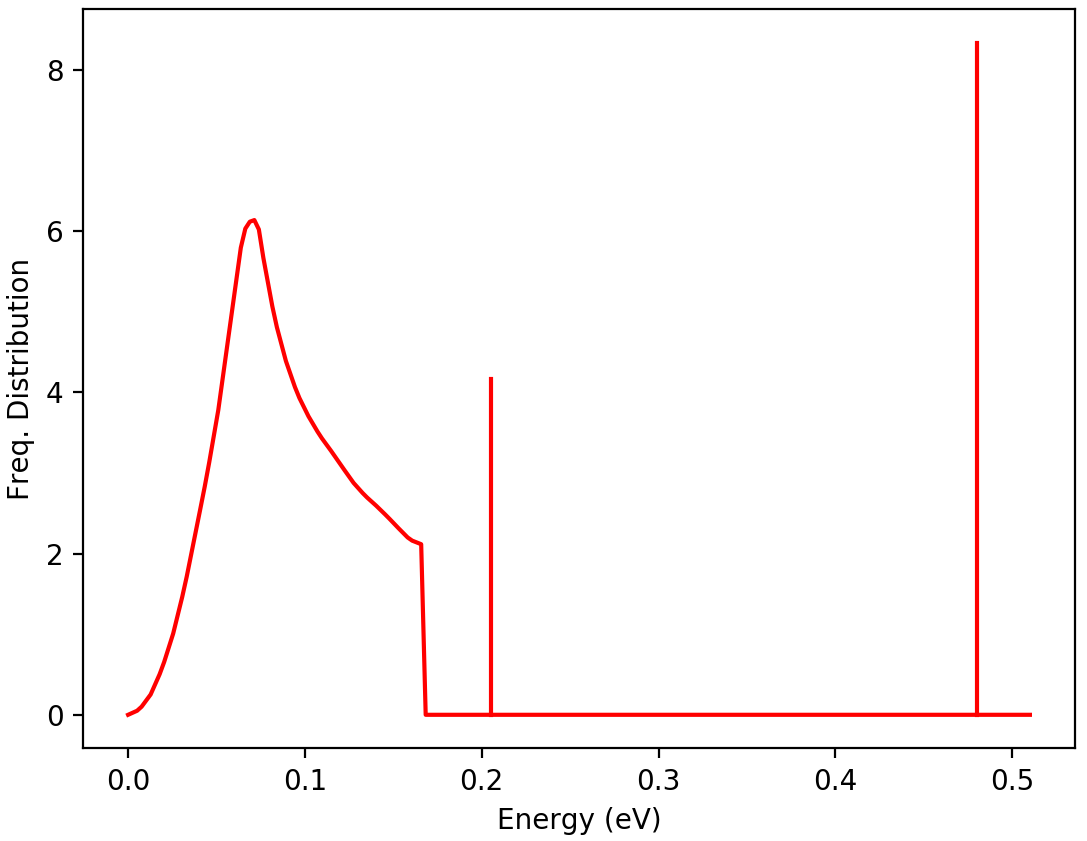
\includegraphics[scale=0.7]{waterPhononDistb}
      \caption[Phonon Distribution for NJOY 2016 Test Problem 9]{The phonon distribution for NJOY 2016 Test Problem 9 is shown above. It contains a continuous contribution, shown on the lower energy region, and two $\delta$ functions to approximate the higher energy peaks. }
      \label{fig:waterPhonon}
    \end{center}
  \end{figure}

  For Test Problem 9, the continuous region of phonon is defined as $\rho(\beta)=\rho(\Delta E/k_bT)$ for $\Delta E$ spanning from 0-0.16575 eV, where the energy grid is uniformly spaced in increments of 0.00255 eV. The translational contribution to Test Problem 9 is removed $(\omega_t=0)$, and thus the continuous weighting $(\omega_s)$ is increased from 0.444444 to 0.5.  The locations and weights of the two discrete oscillators are provided in Table~\ref{tab:test9_delta_facts}. Note that, as required by Eq.\ref{eq:weightsSumTo1}, 
  \begin{equation}
    \omega_s+\omega_1+\omega_2= 0.5 + 0.166667 + 0.333333 = 1.0.
  \end{equation}
  \begin{table}
    \centering
    \caption[Energies and Weights for $\delta$ functions used in NJOY 2016 Test Problem 9]{Energies and Weights for $\delta$ functions used in NJOY 2016 Test Problem 9}
    \label{tab:test9_delta_facts}
    \begin{tabular}{ |c|c| }\hline
      Energy (eV)& Weighting\\\hline
      0.205& 0.166667\\\hline
      0.480 & 0.333333 \\\hline
    \end{tabular}\\[1ex]
  \end{table}



\section{Representing Discrete Oscillators as Continuous Points}
  In order to allow users to avoid the $\delta$ function approximation that is commonly used in NJOY's LEAPR module, it is crucial to demonstrate similar behavior between how the solid-type, continuous treatment vs. discrete oscillator treatment processes sharp peaks. For this discussion, Test Problem 9, which was described in Sec.~\ref{sec:test9} is considered. To allow for more flexible analysis, LEAPR's source code was translated from Fortran to C++. So first, the results of the translated C++ LEAPR are compared against legacy Fortran LEAPR for the simple H in H$_2$O model, to establish validity in the method. Then, the discrete oscillators in Test Problem 9 are replaced with triangles of varying thickness, to illustrate that as the thickness of the triangle decreases, it approaches the behavior characteristic of a $\delta$ function oscillator.
  \subsection{Equivalence of Revised-LEAPR to Legacy-LEAPR}
    NJOY's LEAPR module was translated from Fortran to C++, so as to provide flexibility in later analysis. The C++ translation must of course replicate the original NJOY code adequately. To illustrate this, Fig.~\ref{fig:me_vs_njoy_sab} contains $S(\alpha,\beta)$ as it was calculated using both the original LEAPR code, as well as the translated LEAPR code. Note that the for nearly all $\alpha,\beta$ values shown, the two datasets are virtually indistinguishable from each other. 
    %\begin{figure}[H]
    %  \begin{center}
    %    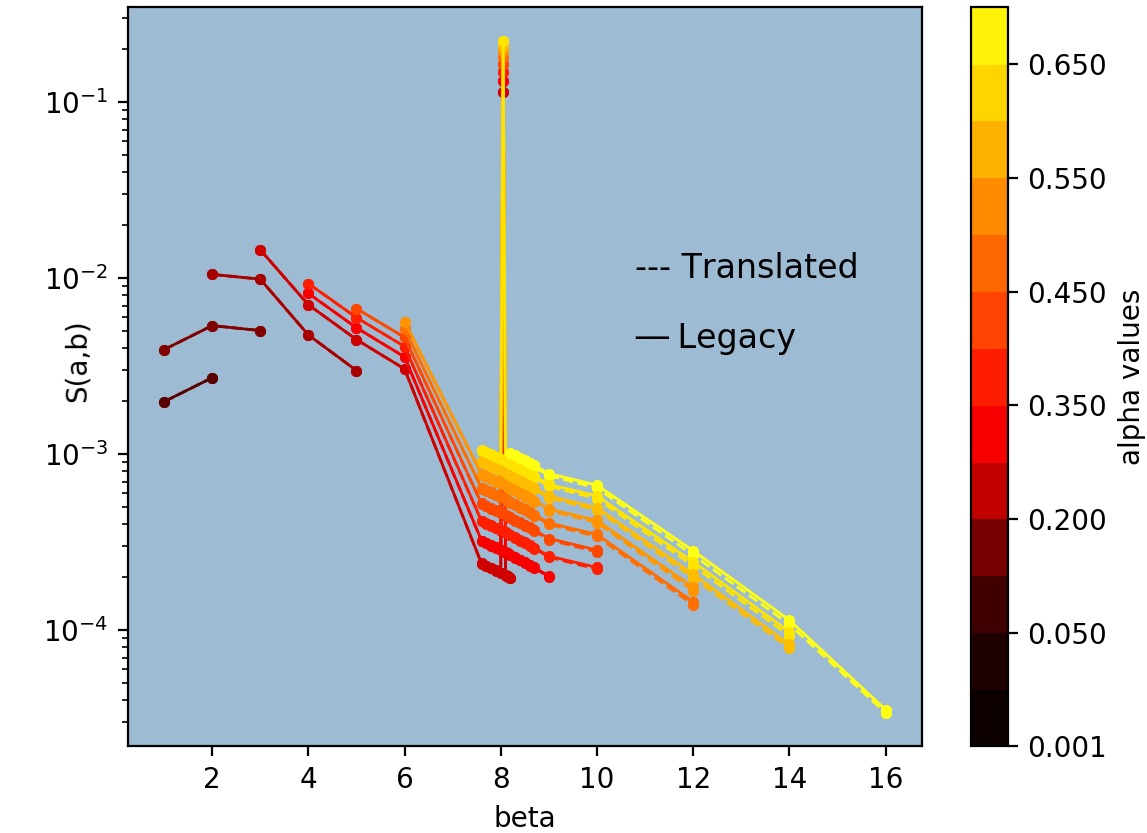
\includegraphics[width=0.75\textwidth]{images/me-vs-njoy-1b}
    %    \caption[Comparison of Translated vs. Legacy LEAPR, for Test \#9 ($S(\alpha,\beta)$)]{Test \#9 $S(\alpha,\beta)$ results, comparing translated vs. legacy LEAPR for H in H$_2$O Test \#9 Input, which are represented using dotted and dashed lines, respectively.}
    %    \label{fig:me_vs_njoy_sab}
    %%  \end{center}
    %\end{figure}
    \begin{figure}[H]
      \begin{center}
        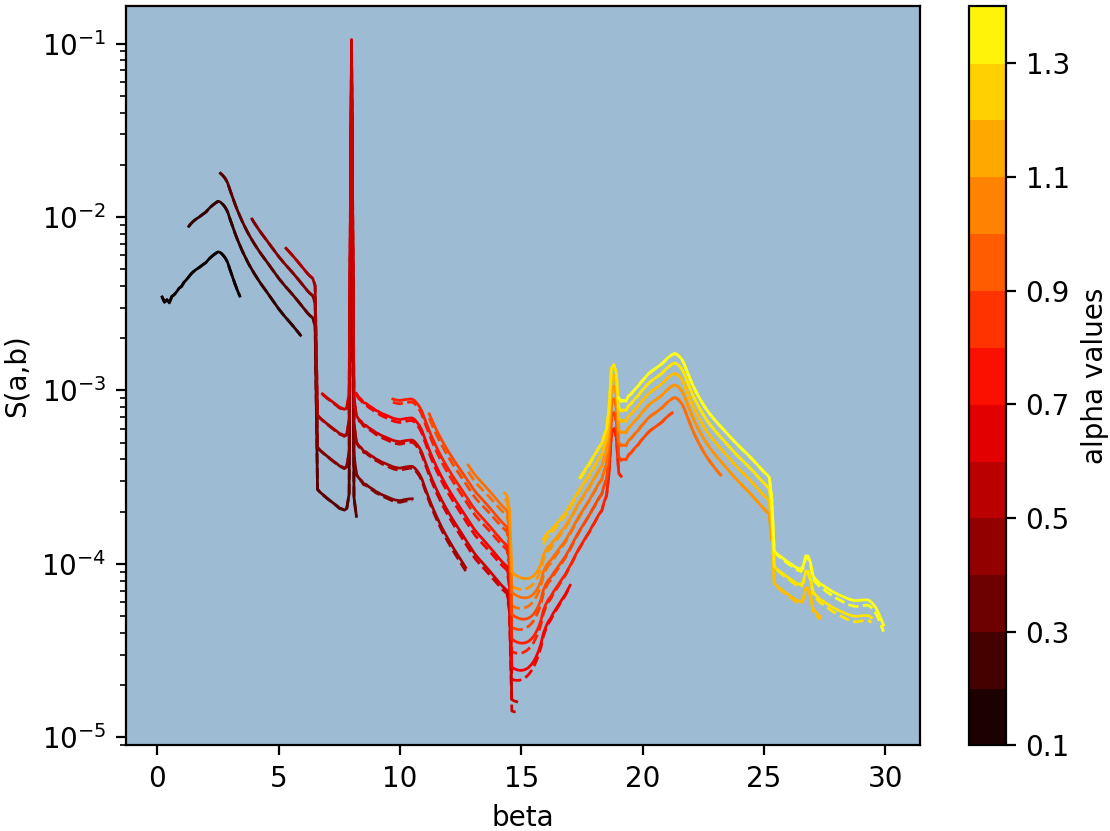
\includegraphics[width=0.85\textwidth]{images/me-vs-njoy-1c}
        \caption[Comparison of Translated vs. Legacy LEAPR, for Test \#9 ($S(\alpha,\beta)$)]{Test \#9 $S(\alpha,\beta)$ results, comparing translated vs. legacy LEAPR for H in H$_2$O Test \#9 Input, which are represented using dotted and dashed lines, respectively. Note the sharp peaks that characterize the $S(\alpha,\beta)$ plots, which correspond to sum values in Eq.~\ref{eq:finalDelta}. They are located at 7.99, 18.79, 26.79, 15.99 eV which correspond to  }
        \label{fig:me_vs_njoy_sab}
      \end{center}
    \end{figure}




    %\begin{figure}[H]
    %  \begin{center}
    %    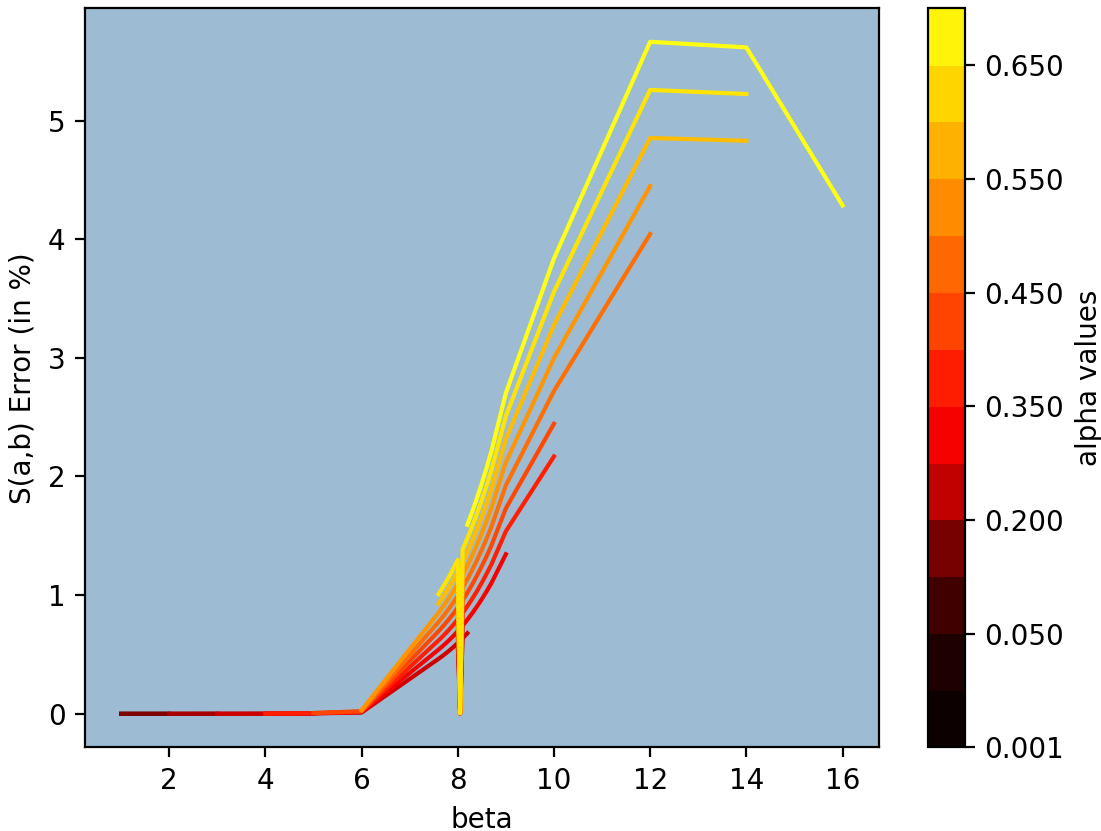
\includegraphics[width=0.75\textwidth]{images/me-vs-njoy-3b}
    %    \caption[Comparison of Translated vs. Legacy LEAPR, for Test \#9 (\% Error) ]{Comparison of translated vs. legacy LEAPR, for test \#9, with the percent error plotted. Note that in the $\beta$ region where percent error increases, is the same region in Fig.~\ref{fig:me_vs_njoy_sab} where the $S(\alpha,\beta)$ values become significantly smaller.}
    %    \label{fig:me_vs_njoy_error}
    %  \end{center}
    %\end{figure}
    \begin{figure}[H]
      \begin{center}
        %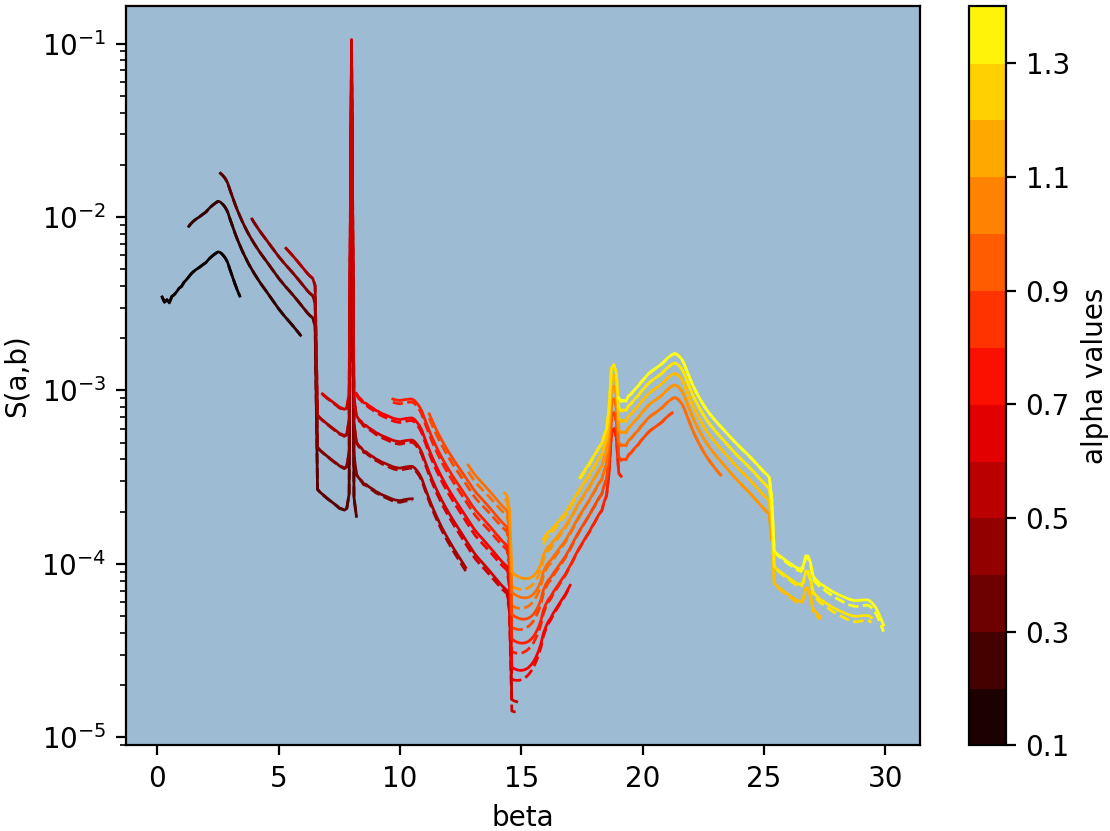
\includegraphics[width=0.70\textwidth]{images/me-vs-njoy-1c}
        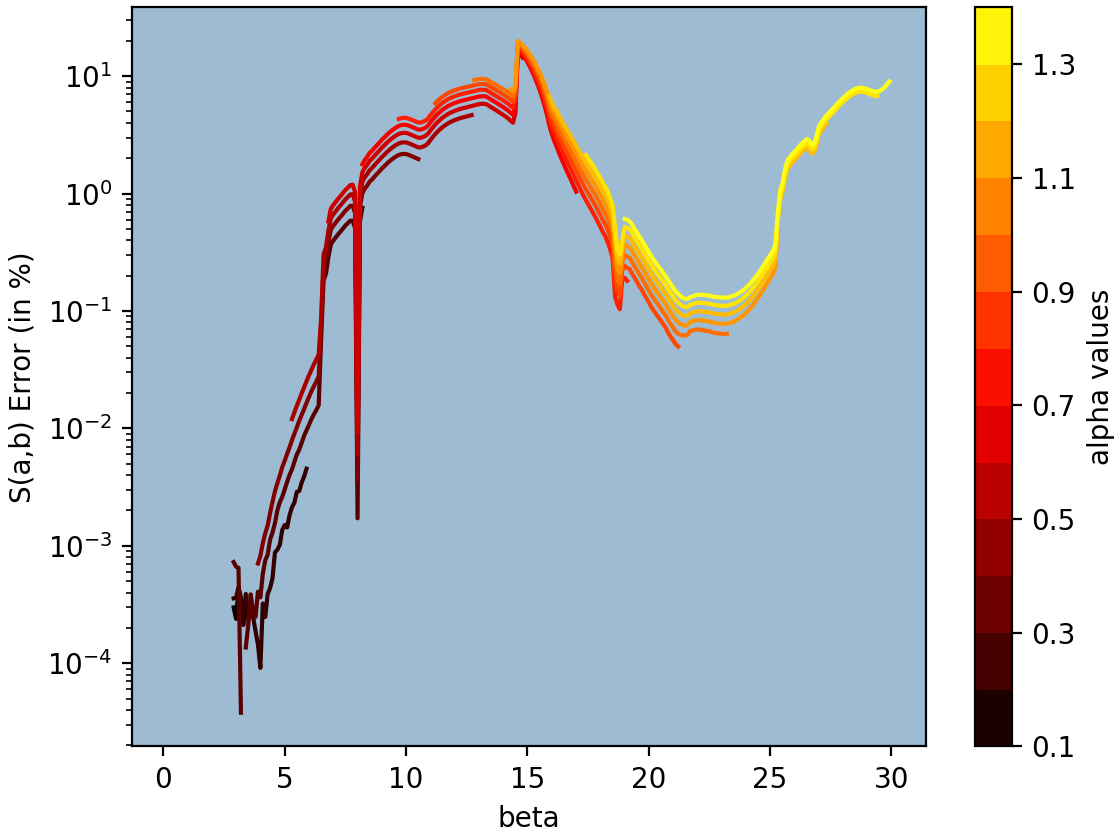
\includegraphics[width=0.75\textwidth]{images/me-vs-njoy-3c}
        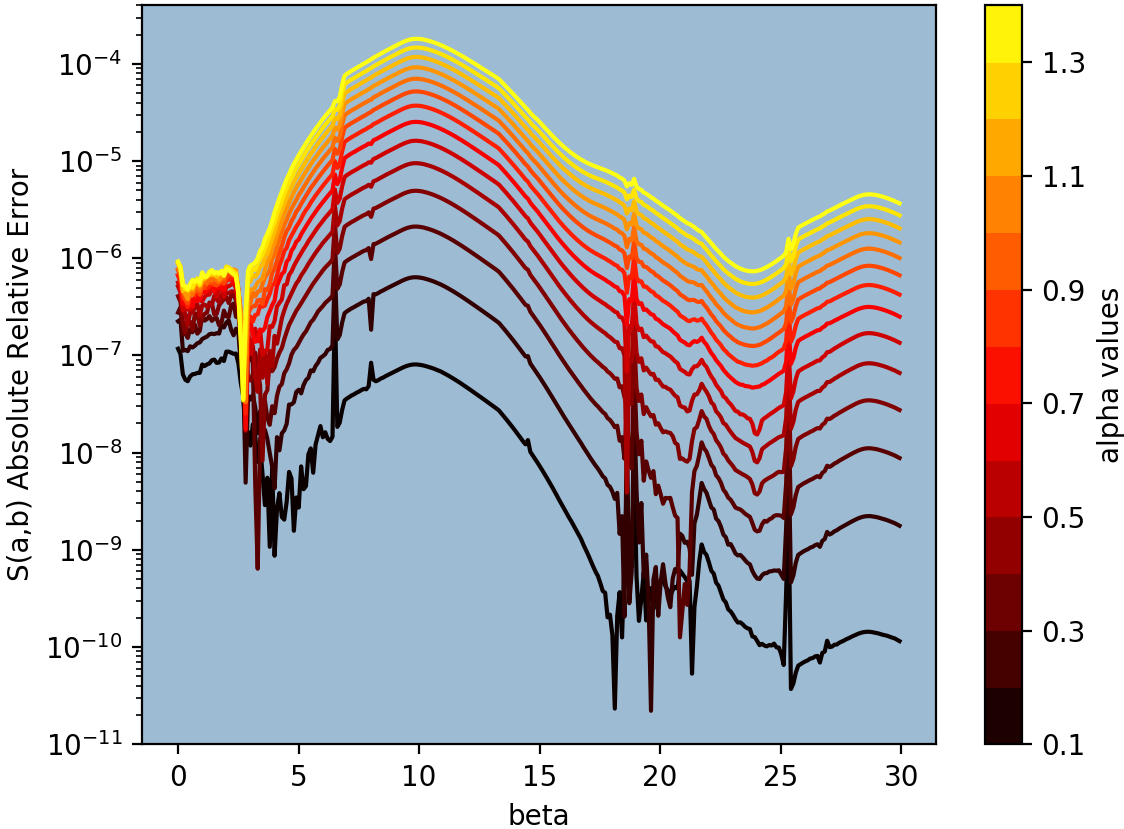
\includegraphics[width=0.75\textwidth]{images/me-vs-njoy-4c}
        \caption[Comparison of Translated vs. Legacy LEAPR, for Test \#9 (\% Error) ]{Comparison of translated vs. legacy LEAPR, for test \#9, with the percent error plotted. Note that in the $\beta$ region where percent error increases, is the same region in Fig.~\ref{fig:me_vs_njoy_sab} where the $S(\alpha,\beta)$ values become significantly smaller.}
        \label{fig:me_vs_njoy_error}
      \end{center}
    \end{figure}



    Fig.~\ref{fig:me_vs_njoy_error} shows the percent error between the $S(\alpha,\beta)$ values produced by the translated and original LEAPR, that were plotted in Fig.~\ref{fig:me_vs_njoy_sab}.  Notice that the percent error is significantly lower in the $\beta$ regions where $S(\alpha,\beta)$ is of reasonable size. 

    Thus, the translated version of LEAPR is considered an adequate tool for processing thermal data for the following discussion. However, conclusions drawn using the translated LEAPR will be verified alongside those drawn from the legacy LEAPR. Note that the translated LEAPR was also tested against legacy LEAPR with other cases considered.


  \subsection{Replacing Discrete Oscillator $\delta$ Functions as Triangles}
    To verify that discrete oscillator treatment can be replicated by using increasingly thin triangles, each triangle must integrate to the weight of its corresponding $\delta$ function. Triangles of various widths (2,4,6,8, and 10 grid spaces) are used to replace both $\delta$ functions, and are plotted in Fig.~\ref{fig:waterPhononTriangle}.
    \begin{figure}[h]
      \begin{center}
        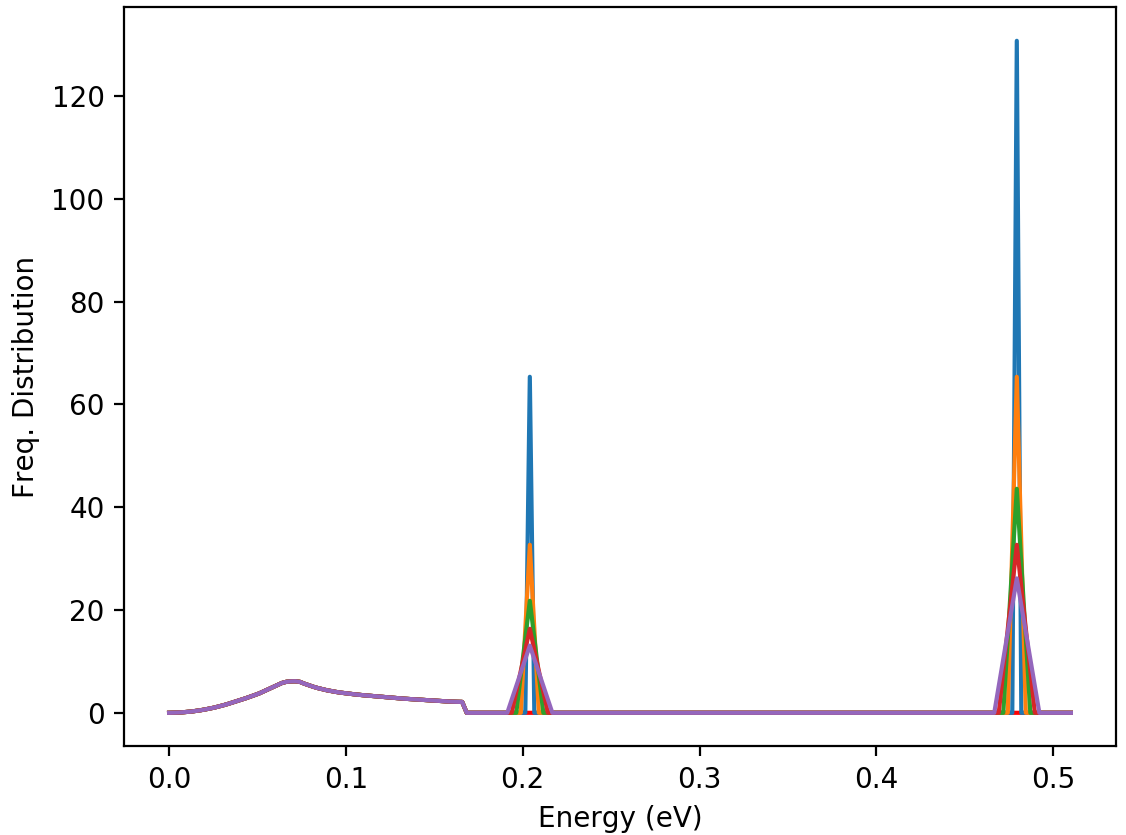
\includegraphics[width=0.8\textwidth]{waterPhononDistTrianglesb}
        %\caption[Phonon Distribution for H in H$_2$O, with oscillators replaced with phonon distribution triangles of various widths]{Phonon Distribution for H in H$_2$O, with oscillators replaced with phonon distribution triangles of various widths. The area under each triangle integrates to its corresponding $\delta$ function weight $\omega_i$, and the lower energy continuous component integrates to the solid-type weight $\omega_s$.}
        \caption[Triangles of various widths approximatin $\delta$ functions for H in H$_2$O]{Phonon Distribution for H in H$_2$O, with oscillators replaced with phonon distribution triangles of various widths. The area under each triangle integrates to its corresponding $\delta$ function weight $\omega_i$, and the lower energy continuous component integrates to the solid-type weight $\omega_s$.}
        \label{fig:waterPhononTriangle}
      \end{center}
    \end{figure}

    NJOY requires any continuous phonon distribution to be provided with respect to a uniformly-spaced energy grid. Thus, in Fig.~\ref{fig:waterPhononTriangle}, the centers of the triangles are not necessarily equal to the exact location of the $\delta$ functions that are specified in Table.~\ref{tab:test9_delta_facts}. A closer view of Fig.~\ref{fig:waterPhononTriangle}, shown in Fig.~\ref{fig:waterPhononTriangleZoomed}, illustrates an offset between the triangle centers and the real oscillator location. Since the triangles' points are limited to increments of $\Delta E=0.00255$ eV, some inaccuracies are to be expected.

    \begin{figure}[h]
      \begin{center}
        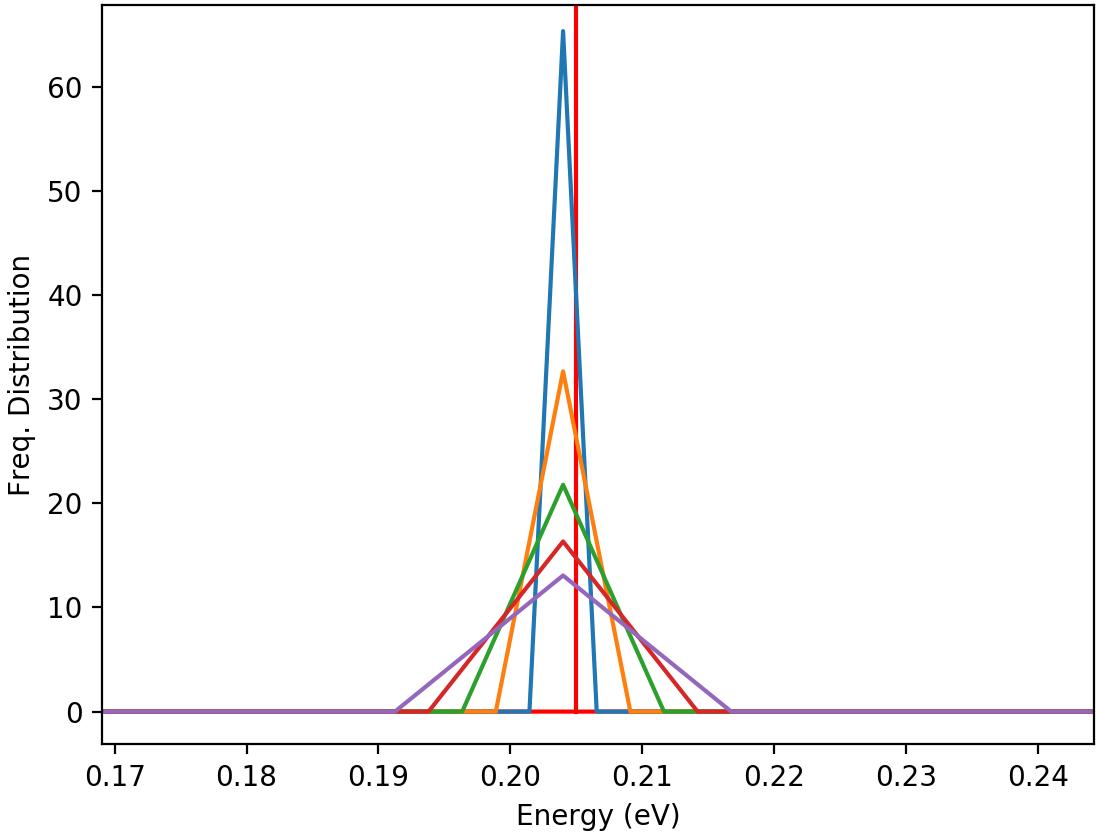
\includegraphics[width=0.7\textwidth]{waterPhononDistTrianglesZoomedb}
        \caption[Close-up of various triangles approximating 0.204 eV $\delta$ function]{This is a zoomed in version of Fig.~\ref{fig:waterPhononTriangle}, where we focus in on the 0.204 eV $\delta$ function. The red line represents the $\delta$ function that is defined in the test \#9, while other colors represent triangles used to approximate the $\delta$ function.}
        \label{fig:waterPhononTriangleZoomed}
      \end{center}
    \end{figure}
    As a result of the discrepancy between discrete oscillator location and triangle center location, the oscillators energies are shifted slightly to align better with the $\Delta E=0.00255$ eV grid to which NJOY is restricted. The $\delta$ function parameters presented in Table.~\ref{tab:test9_delta_facts} are amended to those in Table.~\ref{tab:amended_delta_facts}



    \begin{table}[H]
      \centering
      \caption[Energies and Weights for $\delta$ functions, Amended to Align with Continuous Energy Grid]{Energies and Weights for $\delta$ functions, Amended to Align with Continuous Energy Grid}
      \label{tab:amended_delta_facts}
      \begin{tabular}{ |c|c| }\hline
        Energy (eV)& Weighting\\\hline
        0.204& 0.166667\\\hline
        0.4794 & 0.333333 \\\hline
      \end{tabular}\\[1ex]
    \end{table}

    By slightly shifting the locations of the oscillators so that they are aligned with the triangles' grids, Fig.~\ref{fig:waterPhononTriangleZoomed} now becomes Fig.~\ref{fig:waterPhononTriangleZoomedShifted}. The oscillator energies detailed in Table~\ref{tab:amended_delta_facts} are the problem specifications used for the remainder of this discussion. The phonon distribution defined in Test \#9, which has defined, non-zero values for energies up to 0.16575 eV, is combined with the appropriately sized triangles, and compared against the typical Test \#9 results. 


    \begin{figure}[h]
      \begin{center}
        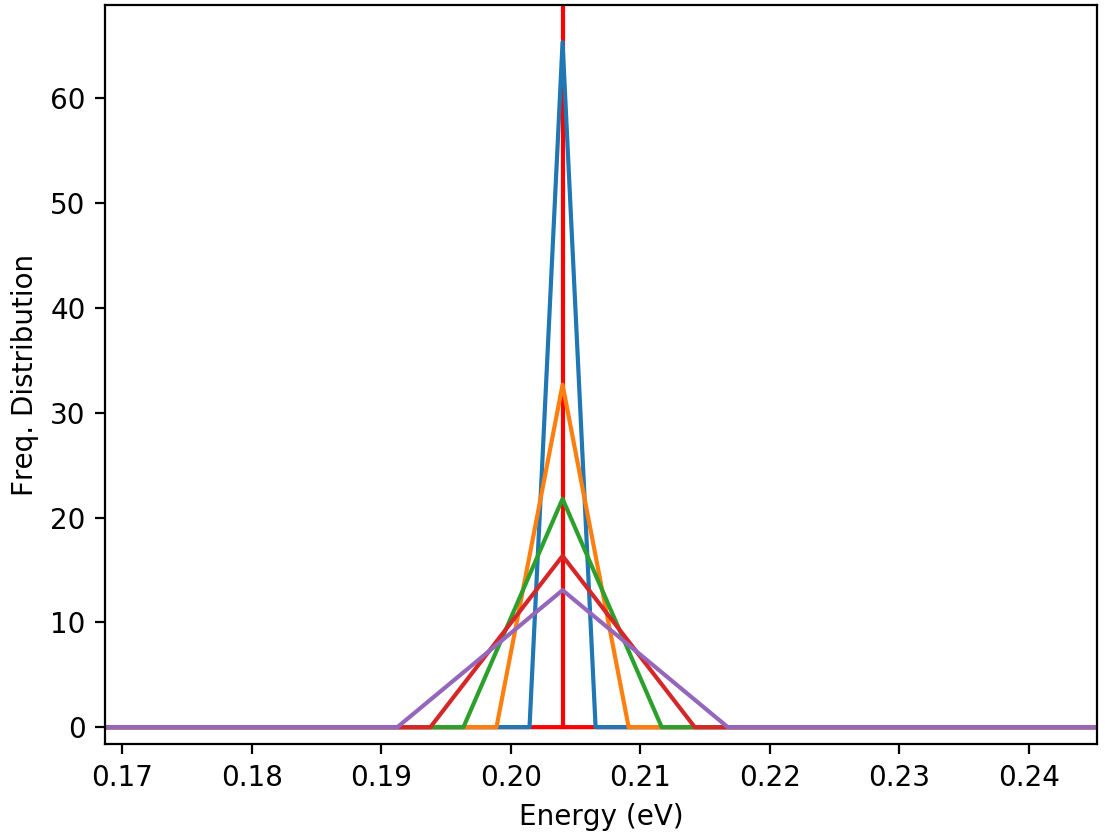
\includegraphics[width=0.7\textwidth]{alteredDeltaZoomedb}
        %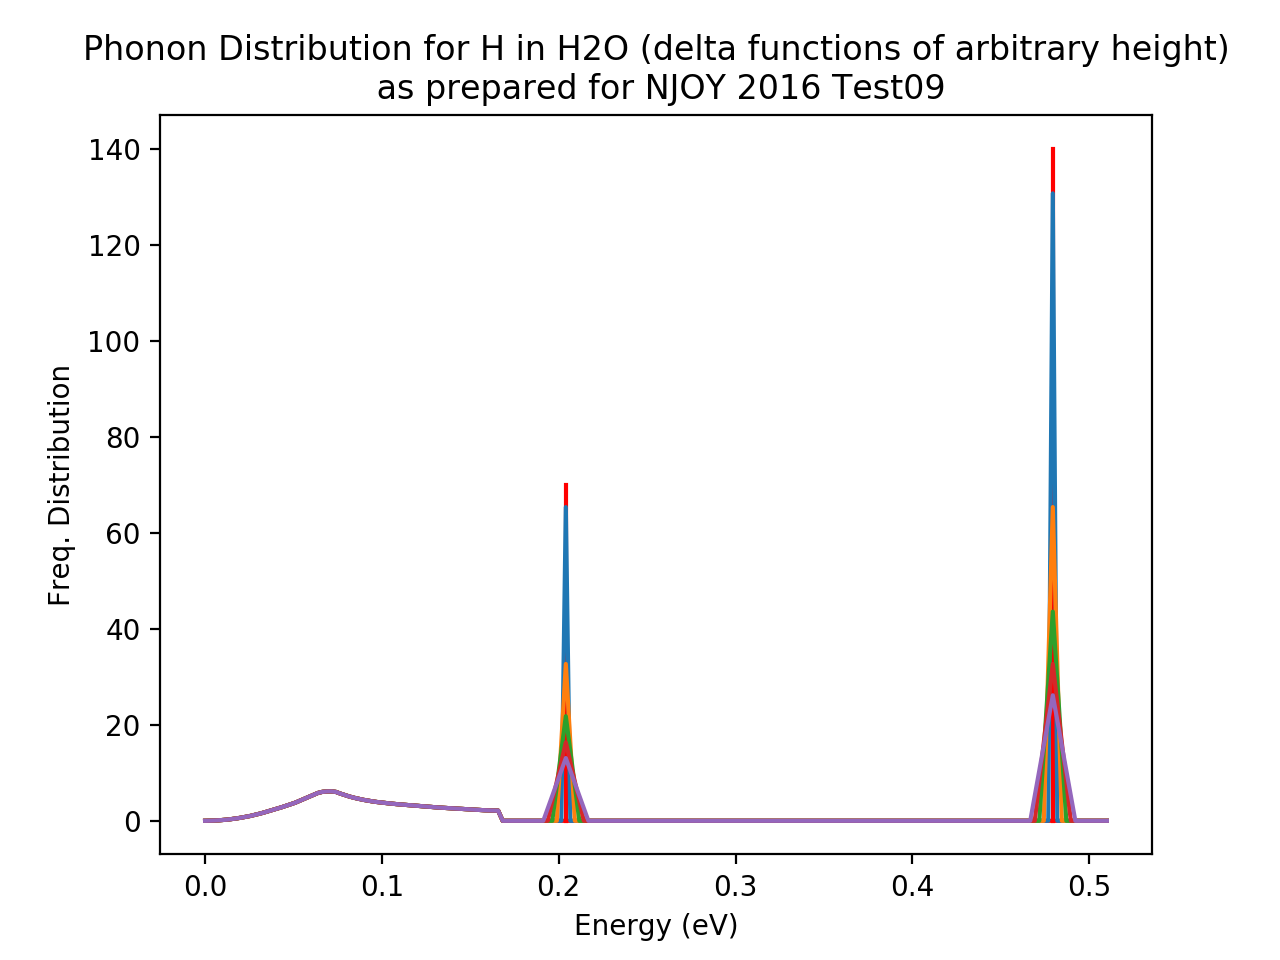
\includegraphics[scale=0.5]{alteredDelta}
        \caption[Triangles of various widths, plotted alongside shifted $\delta$ functions]{Fig.~\ref{fig:waterPhononTriangleZoomed} illustrates an offset between the triangle centers and the $\delta$ function location, due to restrictions in the $\rho(E)$ grid. Thus, $\delta$ function locations were shifted to the energies detailed in Table~\ref{tab:amended_delta_facts}. Thus, Fig.~\ref{fig:waterPhononTriangleZoomed} is amended to the above.}
        \label{fig:waterPhononTriangleZoomedShifted}
      \end{center}
    \end{figure}






\section{$S(\alpha,\beta)$ Response to Continuous vs. Discrete Oscillator Representation} 

  \subsection{$S(\alpha,\beta)$ Response to Thin Triangle vs. Oscillator}\label{sec:thin_triangle_vs_delta}
    The phonon distributions presented in Fig.~\ref{fig:waterPhononTriangle} are input into LEAPR, and the resultant $S(\alpha,\beta)$ is collected. This is compared against the $S(\alpha,\beta)$ grid that is resultant of the typical discrete oscillator representation for the higher end of the H in H$_2$O frequency distribution. As mentioned in Sec.~\ref{sec:test9}, the phonon grid is defined with a uniform energy spacing of $\Delta E=0.00255$  eV, which means that the thinnest triangle available has a total width of $2\times\Delta E=0.0051$ eV. For the remainder of Sec.~\ref{sec:thin_triangle_vs_delta}, this minimum-width triangle will be the only triangle of focus. In Sec.~\ref{sec:vary_triangle_width}, the effects of changing triangle width will be explored.
    Fig.~\ref{fig:sabThinTriangleAllAB} shows the $S(\alpha,\beta)$ grids generated by translated LEAPR, using both the discrete oscillator and the thin triangle phonon representation. The $S(\alpha,\beta)$ grid is plotted against $\beta$ for various $\alpha$ values. There is little discernible difference between the two datasets, so a closeup on the $\beta\approx8$ peak is provided in Fig.~\ref{fig:sabThinTriangleAllABZoomed}.

    \begin{figure}[h]
      \begin{center}
        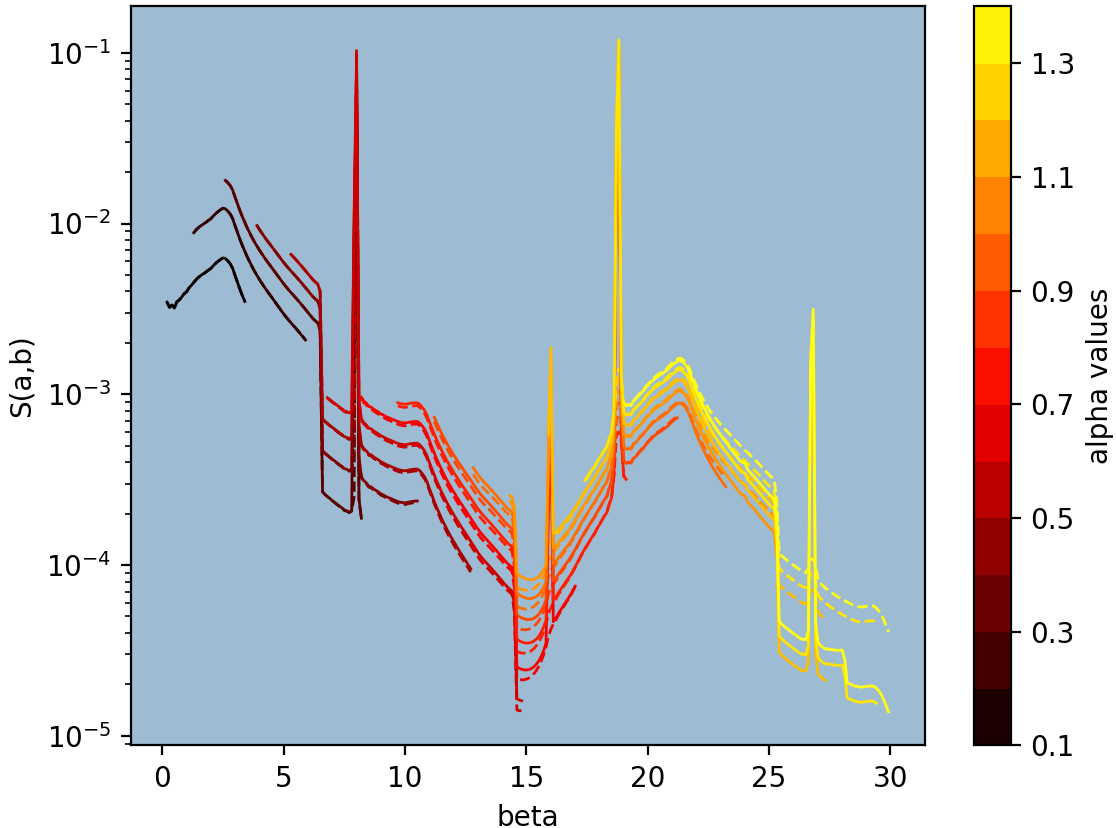
\includegraphics[width=0.7\textwidth]{sab_thinTriangle_and_delta_all_ABb}
        \caption[$S(\alpha,\beta)$ grid, comparing oscillator vs. thin triangle representation (translated LEAPR used)]{$S(\alpha,\beta)$ generated from the translated LEAPR is plotted above, where the discrete oscillator and thin triangle representations are shown using dotted and solid lines, respectively.}
        \label{fig:sabThinTriangleAllAB}
      \end{center}
    \end{figure}



    \begin{figure}[h]
      \begin{center}
        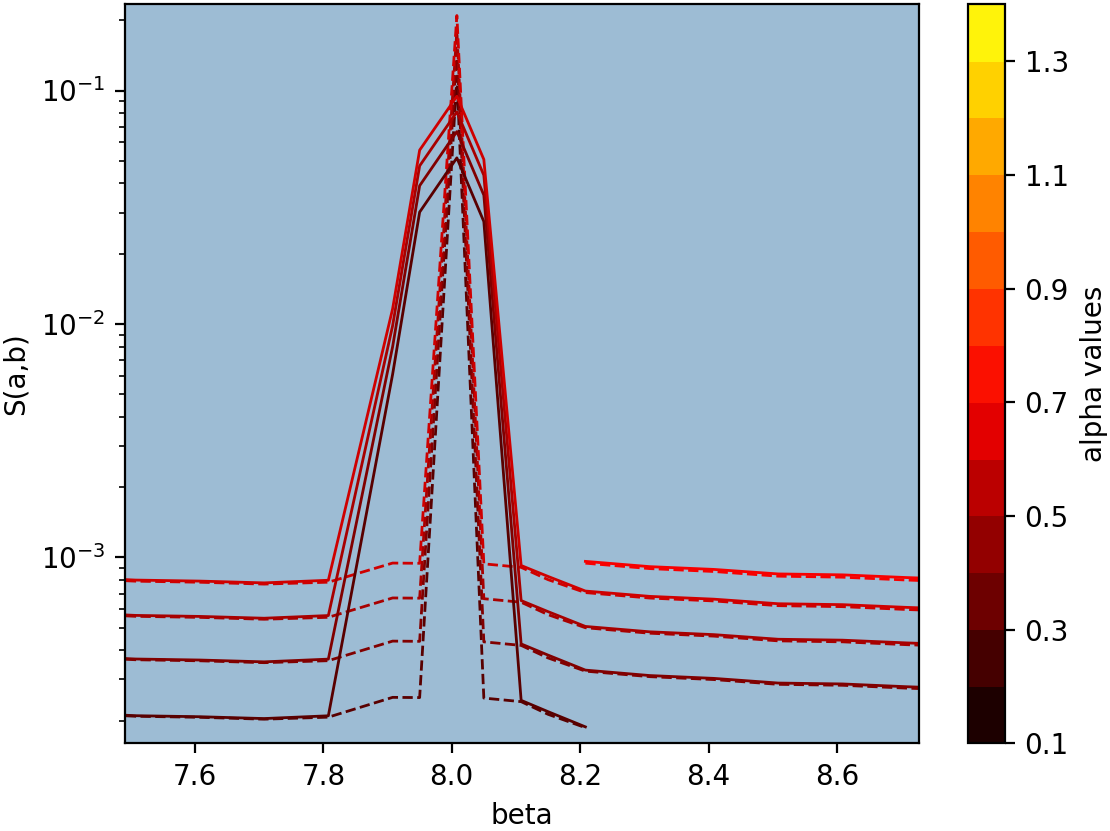
\includegraphics[width=0.7\textwidth]{sab_thinTriangle_and_delta_all_AB_Zoomedb}
        \caption[Close-up view of $S(\alpha,\beta)$ grid that compares oscillator vs. thin triangle representation (translated LEAPR used)]{$S(\alpha,\beta)$ generated from the translated LEAPR is plotted above, where the discrete oscillator and thin triangle representations are shown using dotted and solid lines, respectively. This is a close-up view of Fig.~\ref{fig:sabThinTriangleAllAB}.}
        \label{fig:sabThinTriangleAllABZoomed}
      \end{center}
    \end{figure}
    Looking at Fig.~\ref{fig:sabThinTriangleAllABZoomed}, it is apparent that the continuous representation of the peak has a wider spread than that of the discrete oscillator. This is to be expected, since the triangle needs three points in the frequency distribution to define its shape, while the $\delta$ function is defined at one particular point. 



    %\begin{figure}[h]
    %  \begin{center}
    %    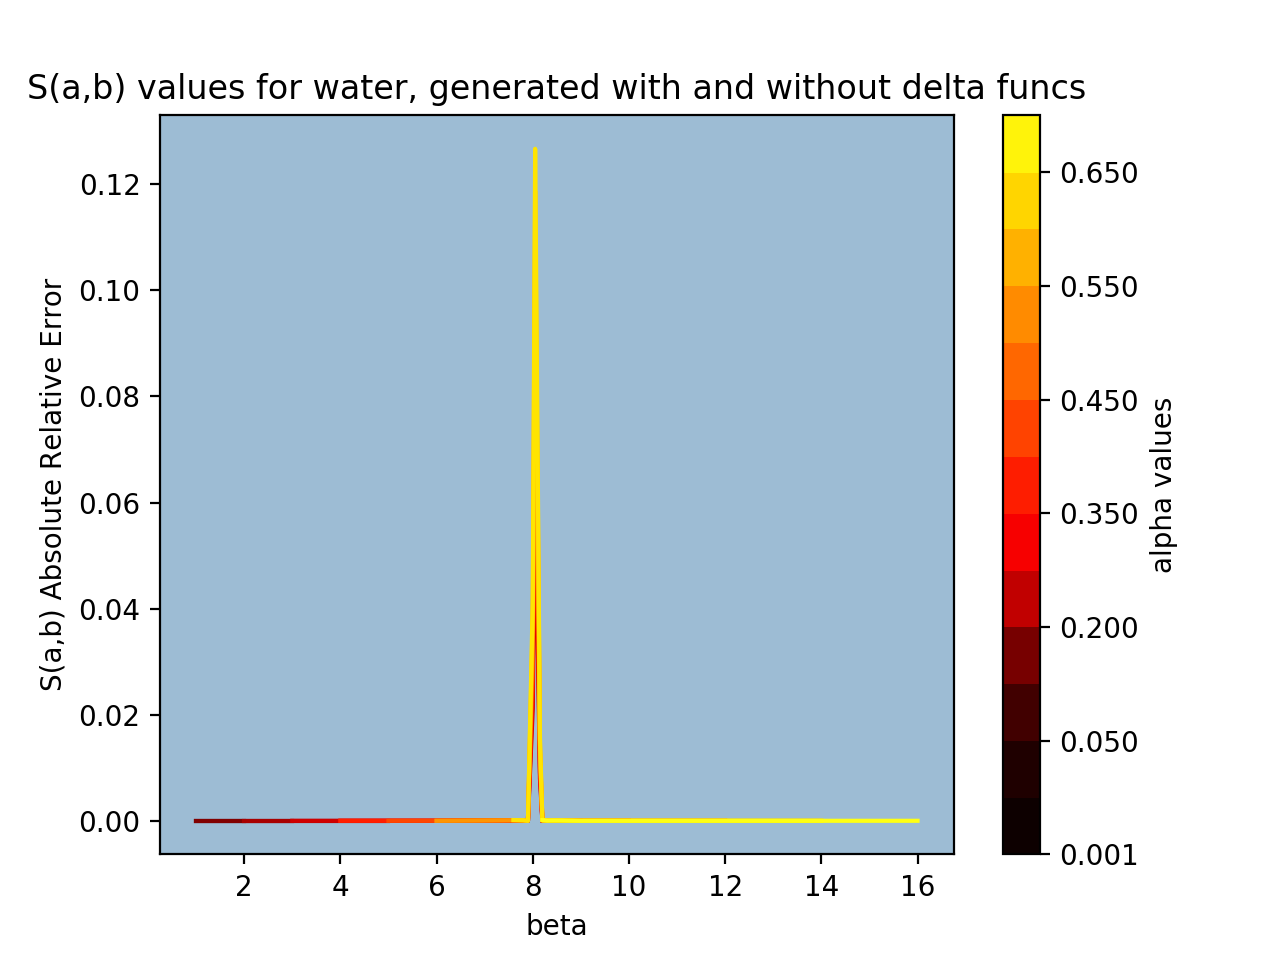
\includegraphics[scale=0.6]{sab_thinTriangle_error}
    %    \caption{This is the absolute relative error between the $S(\alpha,\beta)$ produced using $\delta$ functions and $S(\alpha,\beta)$ produced using a thin (width = 2 spaces) triangle. Note that the error is very small away from the $\beta\approx8.05$ peak. }
    %    \label{fig:sabThinTriangleError}
    %  \end{center}
    %\end{figure}







    
    \clearpage

  \subsection{$S(\alpha,\beta)$ Response to Changes in Triangle Size}\label{sec:vary_triangle_width}



    \subsection*{Results: Triangles of Various Widths vs. $\delta$ Func.}

    \begin{figure}[h]
      \begin{center}
        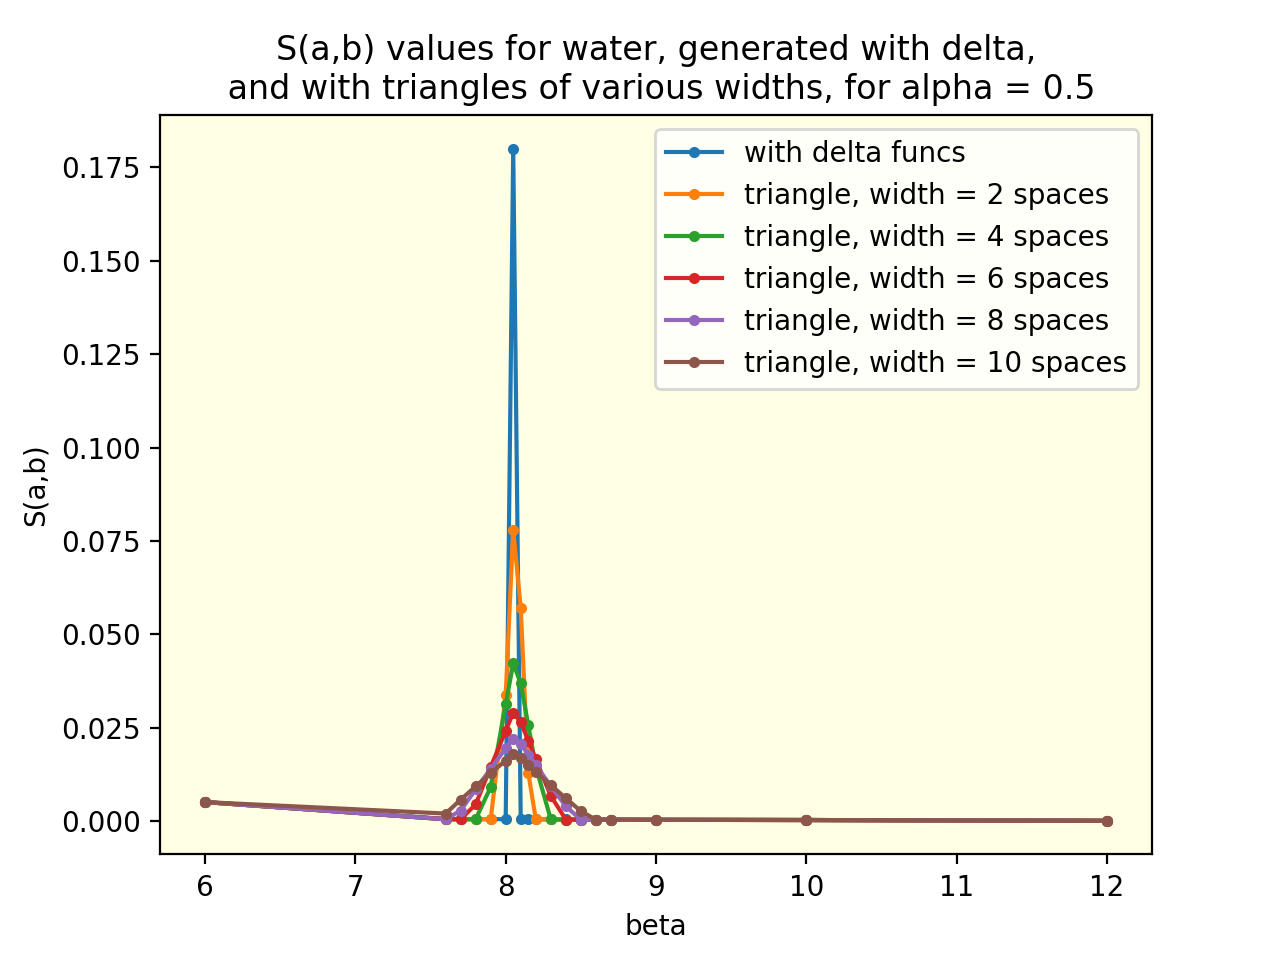
\includegraphics[scale=0.6]{diff_widths_alpha_0p5}
        \caption{}
        \label{fig:diff_widths_alpha_0p5}
      \end{center}
    \end{figure}


    We also look at the total error.
    \[E_{total}=\sum_{\beta}\sum_\alpha \Big|S^\delta(\alpha,\beta)-S^\triangleleft(\alpha,\beta)\Big|\]

    \begin{figure}[h]
      \begin{center}
        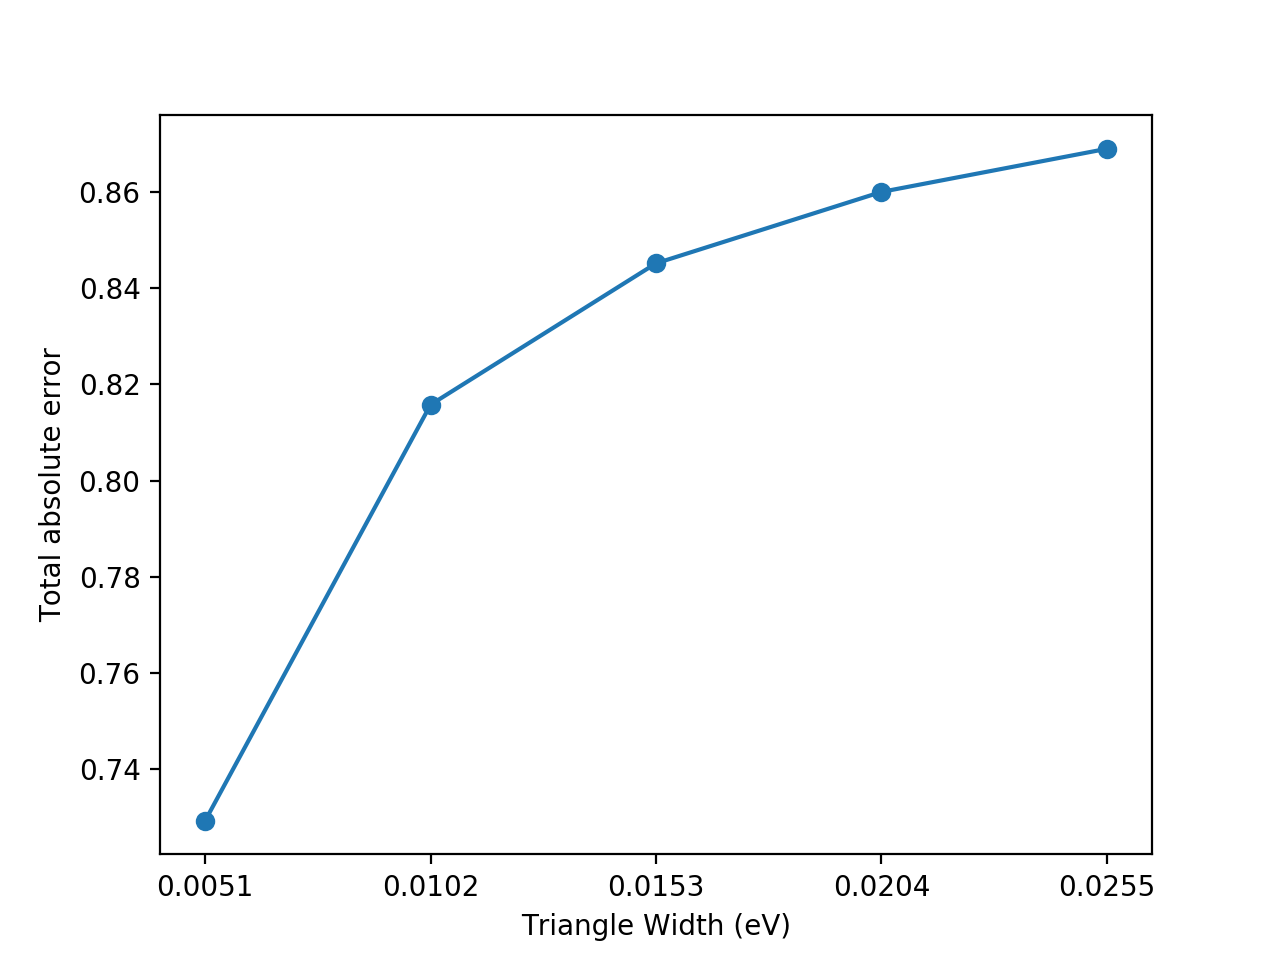
\includegraphics[scale=0.6]{diff_widths_total_error}
        \caption{Note that as the width of the triangle decreases, the total accumulated error decreases significantly.}
        \label{fig:diff_widths_total_error}
      \end{center}
    \end{figure}






          \clearpage
\section{Nonuniform Phonon Distribution Energy Grid}



\end{document}
